\subsection{HDR ML Anomaly Challenge (Sea Level Rise)}
{{\footnotesize
\noindent A challenge combining North Atlantic sea-level time-series and satellite imagery to detect flooding anomalies. Models submitted via Codabench. 


\begin{description}[labelwidth=4cm, labelsep=1em, leftmargin=4cm, itemsep=0.1em, parsep=0em]
  \item[date:] 2025-03-03
  \item[version:] v1.0
  \item[last\_updated:] 2025-03
  \item[expired:] unknown
  \item[valid:] yes
  \item[valid\_date:] 2025-03-03
  \item[url:] \href{https://www.codabench.org/competitions/3223/}{https://www.codabench.org/competitions/3223/}
  \item[doi:] 10.48550/arXiv.2503.02112
  \item[domain:] Climate Science; Time-series, Image/CV
  \item[focus:] Detecting anomalous sea-level rise and flooding events via time-series and satellite imagery
  \item[keywords:]
    - anomaly detection
    - climate science
    - sea-level rise
    - time-series
    - remote sensing
  \item[licensing:] NA
  \item[task\_types:]
    - Anomaly detection
  \item[ai\_capability\_measured:]
    - Detection of environmental anomalies
  \item[metrics:]
    - ROC-AUC
    - Precision/Recall
  \item[models:]
    - CNNs, RNNs, Transformers
  \item[ml\_motif:]
    - Time-series, Image/CV
  \item[type:] Dataset
  \item[ml\_task:]
    - Anomaly detection
  \item[solutions:] Solution details are described in the referenced paper or repository.
  \item[notes:] Sponsored by NSF HDR; integrates sensor and satellite data. 

  \item[contact.name:] HDR A3D3 Team
  \item[contact.email:] unknown
  \item[results.links.name:] ChatGPT LLM
  \item[fair.reproducible:] Yes
  \item[fair.benchmark\_ready:] Yes
  \item[id:] hdr\_ml\_anomaly\_challenge\_sea\_level\_rise
  \item[Citations:] \cite{campolongo2025buildingmachinelearningchallenges3}
\end{description}

{\bf Ratings:} ~ \\

\begin{tabular}{p{0.15\textwidth} p{0.07\textwidth} p{0.7\textwidth}}
\hline
Rating & Value & Reason \\
\hline
dataset & 5 & Uses preprocessed, public, and well-structured sensor and satellite data for the
North Atlantic sea-level rise region.
 \\
documentation & 5 & Challenge page, starter kits, and related papers offer strong guidance for participants.
 \\
metrics & 5 & Standard metrics such as ROC-AUC, precision, and recall are specified and suitable
for the anomaly detection tasks.
 \\
reference\_solution & 1 & No starter models or baseline implementations linked or provided publicly.
 \\
software & 2 & Benchmark platform exists on Codabench, but no baseline code or maintained repository
for reference solutions provided yet.
 \\
specification & 5 & Well-defined anomaly detection task combining satellite imagery and time-series data,
with clear physical and domain-specific framing.
 \\
\hline
\end{tabular}

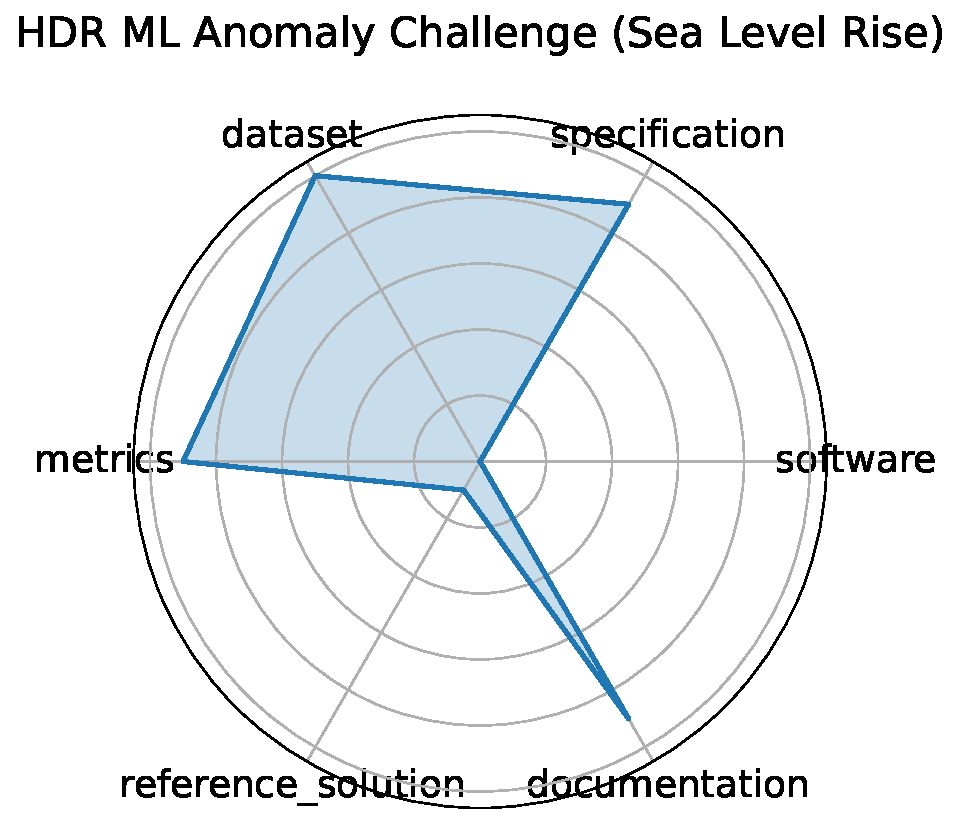
\includegraphics[width=0.2\textwidth]{hdr_ml_anomaly_challenge_sea_level_rise_radar.pdf}
}}
\clearpage